\section*{穿过货场}

出生后先看正前方的行车，再找它右侧的铁皮棚。应急发电机就在棚下。中央车道通往工位，车道中段的电缆会间歇放电。想给瓦特留出拿药和维修的时间，可以往北绕到货柜背后，再从另一端回到棚前。

\begin{center}
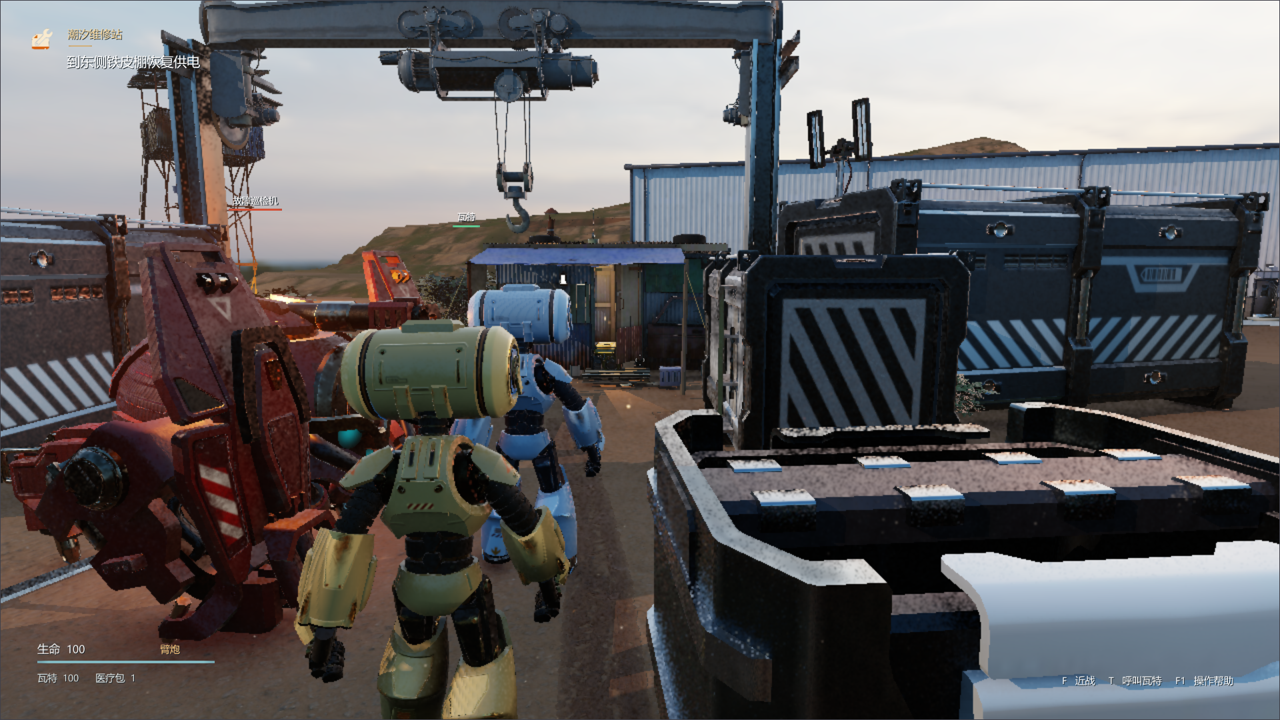
\includegraphics[width=.49\linewidth]{../../../output/validation/station-encounter/routes/central/discharge.png}\hfill
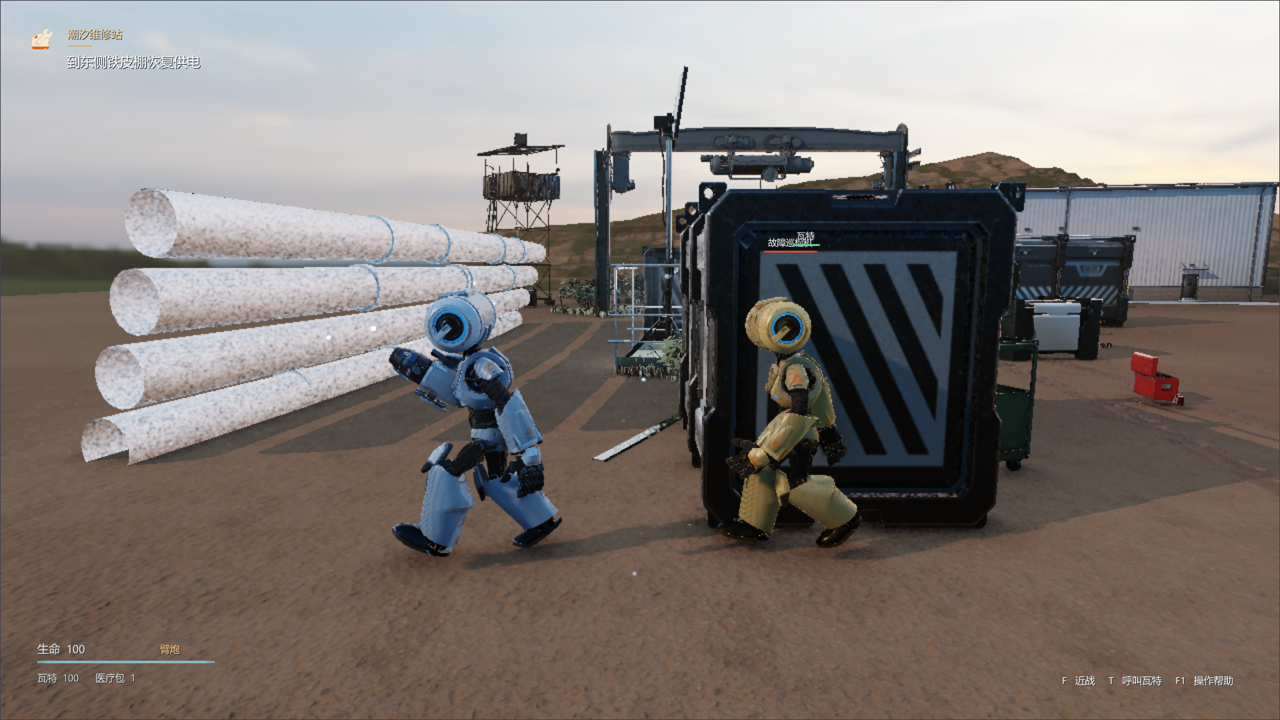
\includegraphics[width=.49\linewidth]{../../../output/validation/station-encounter/routes/north/cover.png}
\end{center}
\picturecaption{同一关卡的两条路线。左图从车道靠近巡检机，右图中蓝色玩家已经绕到货柜另一侧，瓦特正从后面跟上。}

巡检机在两处巡查点之间来回走。它看见维修员才开始靠近，进入放电距离后停下蓄能，橙色灯光逐渐变亮。此时绕过货柜，会让它失去目标并中断本轮蓄能。它先去最后看见人的地方搜索，然后返回巡查路线。供电恢复后，电缆停止放电，西侧闸口亮起通行灯。等瓦特也到闸口就可以撤离。

\begin{center}
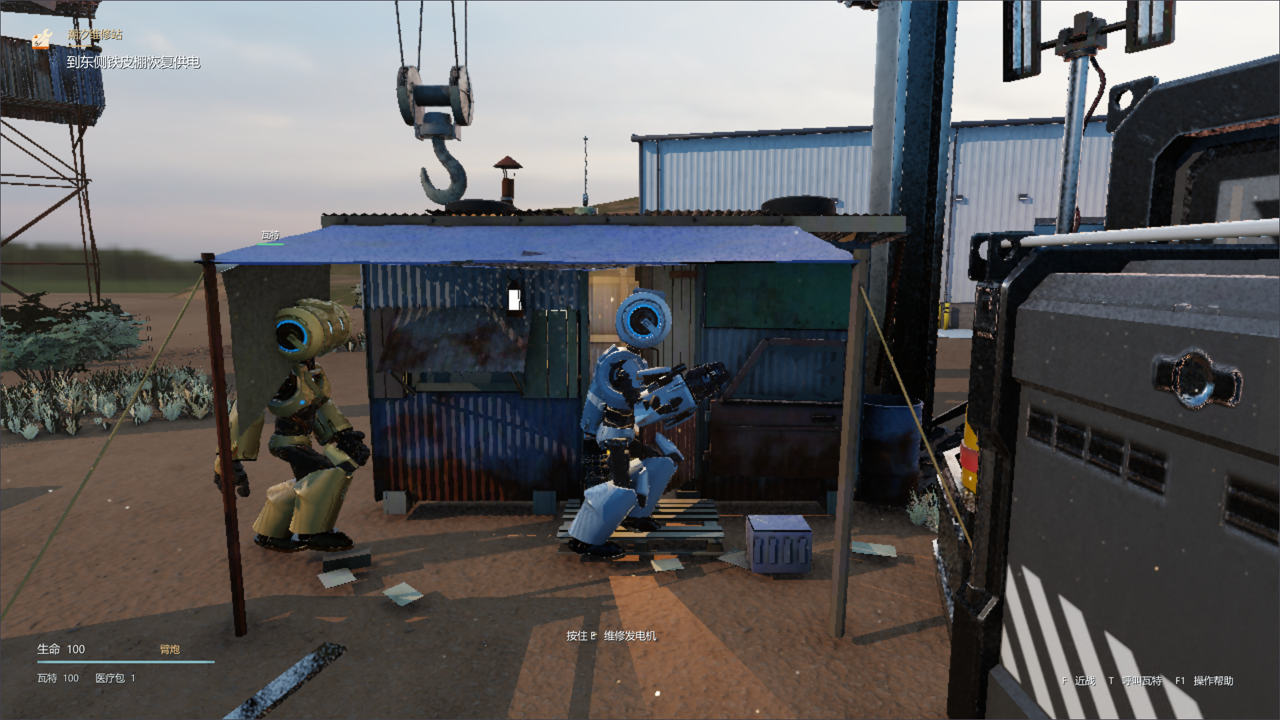
\includegraphics[width=.70\linewidth]{../../../output/validation/station-encounter/routes/north/generator.png}
\end{center}
\picturecaption{从北侧绕行后抵达发电机。靠近设备按住 E，或在队友通讯中请瓦特修理。}

在 Forge 中选中「故障巡检机」，「角色行为树」会显示它当前选择的分支。每组连线从上往下检查，例如进入距离后先看线圈是否还在冷却，再决定蓄能还是放电。选中脚本可以调整感知距离、巡逻端点和蓄能时间。灯的位置和最亮时的强度取自场景中的「巡检机蓄能灯」。
